% TODO: TIRAR LEVE DOS TESTES

\chapter{Plano de testes}
Esse capítulo visa apresentar o plano de testes utilizado no ambiente de execução deste trabalho de conclusão de curso. A primeira seção descreve a infraestrutura virtual e também as configurações do \textit{cluster} \textit{Kubernetes} utilizadas nos testes. Em seguida, são apontados os parâmetros aplicados no ambiente de testes e as métricas de interesse coletadas. Na Seção 4.3 é apresentado o simulador de eventos responsável pelas execuções dos testes em diferentes cenários de erros de escalonamento. Por fim, as considerações parciais são apresentadas.

%Um dos principais desafios do presente trabalho é investigar e definir os parâmetros da arquitetura proposta. A princípio, há dois parâmetros inicias os quais serão desenvolvidos: (1) variação no número de réplicas do escalonador e (2) quantidade de \textit{nodes} do \textit{cluster} que cada \textit{worker} gerenciará. No contexto do presente trabalho, (1) será variado em diversas rodadas de testes, será considerado de início apenas 2 réplicas e subir a quantidade gradativamente até atingir o limite físico da arquitetura. Já (2) possui um nível de complexidade maior que (1), a forma natural é dividir de forma proporcional, por exemplo, em um \textit{cluster} com 10 \textit{nodes} e 5 \textit{workers} então cada \textit{worker} gerenciará 2 \textit{nodes}. Contudo, de acordo com a literatura, esse é um parâmetro que há margem de refinamento. Considera-se o trabalho de \citeonline{vaucher2018sgxaware}, o qual consiste em escalonamento em \textit{cluster} heterogêneo -- máquinas com diferentes arquiteturas e capacidades de processamento. Neste cenário, não seria interessante utilizar o método proporcional de divisão entre \textit{workers} e \textit{nodes}. Outro exemplo é o trabalho de \citeonline{Wang2019Pigeon}, o qual consiste em particionar o \textit{cluster} de acordo com a complexidade das cargas de trabalho. Este trabalho sugere que cargas de trabalho menores devem ser executadas em um segmento do \textit{cluster} diferente que cargas de trabalhos consideradas complexas. Neste cenário houve acréscimo do desempenho na métrica de tempo de espera.

%As métricas de interesse do presente trabalho estão relacionadas com o desempenho de escalonamento em cenários de falhas. Quanto menos tempo uma carga de trabalho permanecer na fila, maior é o desempenho da proposta de escalonamento. Portanto, há duas métricas que serão avaliadas de acordos com os parâmetros propostos: tempo de espera de escalonamento e \textit{makespan}. As métricas de sobrecarga também serão importantes, principalmente relacionadas a sobrecarga do \textit{node}, seja de espaço ou processamento.

\section{Infraestrutura Virtual}
O ambiente de testes foi cedido pela nuvem computacional privada da UDESC em ambiente virtualizado \textit{OpeStack}. Ao todo, possui 20 \textit{vCPUs} e 40 \textit{GB} de memória \textit{RAM}. A partir dos recursos disponíveis foram provisionadas 9 máquinas virtuais \textit{Ubuntu Cloud 20.04 LTS}, para  a construção de um \textit{cluster} \textit{Kubernetes} na versão 1.23.5. As configurações das máquinas do \textit{cluster} são denominadas \textit{m1.medium} (2 \textit{vCPUs} e 4 \textit{GB} de memória \textit{RAM}) e \textit{m1.large} (4 \textit{vCPUs} e 8 \textit{GB} de memória). O \textit{cluster} provisionado possui  2 nós responsáveis pelo \textit{Control Plane} com o objetivo de trabalhar com alta disponibilidade, sendo o nó principal com a configuração \textit{m1.large} e o nó réplica representado por uma instância \textit{m1.medium}. Além disso, há mais 6 máquinas \textit{m1.medium}, sendo 6 nós trabalhadores do \textit{cluster} \textit{Kubernetes} e uma máquina responsável pelo balanceador de carga do \textit{Kube API Server}. A visualização do \textit{cluster} configurado, representado por um conjunto de máquinas virtuais, pode ser visualizado na Figura \ref{fig:openstack}.
\begin{figure}[h!]
	\caption{\label{fig:openstack}Implantação no \textit{OpenStack}}
	\centering
	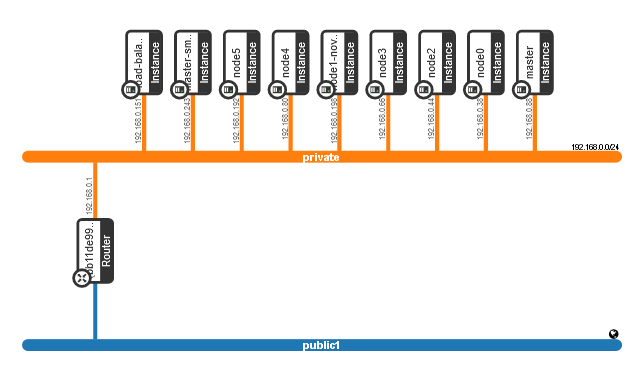
\includegraphics[width=.7\linewidth]{assets/openstack.png}
	\legend{Fonte: O autor}
\end{figure}

\section{Parâmetros e Métricas}
Um dos principais desafios na construção do ambiente experimental é a investigação e as definições de parâmetros e métricas de interesse. Os parâmetros estão relacionados com o ambiente de testes, sendo eles: quantidade total de \textit{pods} submetidos a plataforma (50), quantidade total de simulações de \textit{crashes} de escalonamento (varia de acordo com o cenário de erro que será posteriormente apresentado) e tempo de espera do evento de submissão de \textit{pods} (6 segundos). Este último parâmetro será esclarecido na Seção \ref{sec-simulador-de-eventos}. Já os parâmetros relacionados ao sistema de escalonamento são: quantidade de réplicas do escalonador padrão configurado em alta disponibilidade (1) e quantidade de réplicas dos componentes \textit{Master} (3) e \textit{Worker} (3) do \ac{KMS}.

As métricas de interesse do presente trabalho estão relacionadas com o desempenho de escalonamento em cenários de falhas. Quanto menos tempo uma carga de trabalho permanecer na fila, maior é o desempenho da proposta de escalonamento. Portanto, há duas métricas que serão avaliadas no ambiente de testes de acordos com os parâmetros propostos: tempo de espera de escalonamento e \textit{makespan}.

\section{Simulador de eventos \label{sec-simulador-de-eventos}}
Para analisar as abordagens de escalonamento foi desenvolvido um simulador de eventos discretos com o intuito de exercitar o escalonador. O simulador de eventos possui como parâmetros o total de \textit{pods} que são enviados à plataforma e quantidade total de eventos e erros de escalonamento. As cargas são enviadas para a plataforma de forma gradual respeitando a curva de distribuição normal, com o objetivo de simular um ambiente de produção. No contexto desse simulador, um evento de submissão corresponde a uma quantidade $n$ de \textit{pods} que serão enviados para a plataforma de forma assíncrona, isto é, todos os \textit{pods} de um evento são enviados simultaneamente ao escalonador. Além de enviar \textit{pods}, o simulador também é responsável por simular erros nos sistemas de escalonamento. O erro faz com que o escalonador não esteja disponível por um período de tempo, consequentemente, quanto maior o tempo que o escalonador permanecer indisponível maior será a degradação das métricas de desempenho. 

%Portanto, a técnica de recuperação de falhas e a eficiência da eleição são os pontos determinantes do escalonamento em cenário de falhas.

Os testes realizados consistem em enviar um total de 120 \textit{pods} ao escalonador propagados em 50 eventos de submissões, sendo que cada evento possui duração de 6 segundos e são executados de forma síncrona. Isto é, um evento inicia sua execução apenas após o término da execução do evento anterior. Os \textit{pods} submetidos à plataforma foram construídos para estressar o consumo de memória, visto que mensurar uma alocação válida de \textit{CPU} é um processo complexo por se tratar de um valor excepcionalmente volátil. Logo, as foram definidos como requisitos de recursos computacionais $128$\textit{MiB} de memória \textit{RAM} sem uma  quantidade mínima de \textit{vCPU}. O gráfico que representa o modelo padrão dos testes é exibido na Figura \ref{fig:workload-distribution}.

% Em um cenário ideal as métricas de escalonamento de um \textit{Pod} representam aproximadamente: \textit{wait time} de $2,5s$, \textit{makespan} de $28s$ e tempo de execução de $25s$. A cada teste são submetidos 100 \textit{pods} e representam uma requisição de recursos totais de $12,8 GB$ de memória e $25,0$ de tempo de ${vCPU}$

\begin{figure}[h!]
	\caption{\label{fig:workload-distribution} Gráfico de submissões}
	\centering
	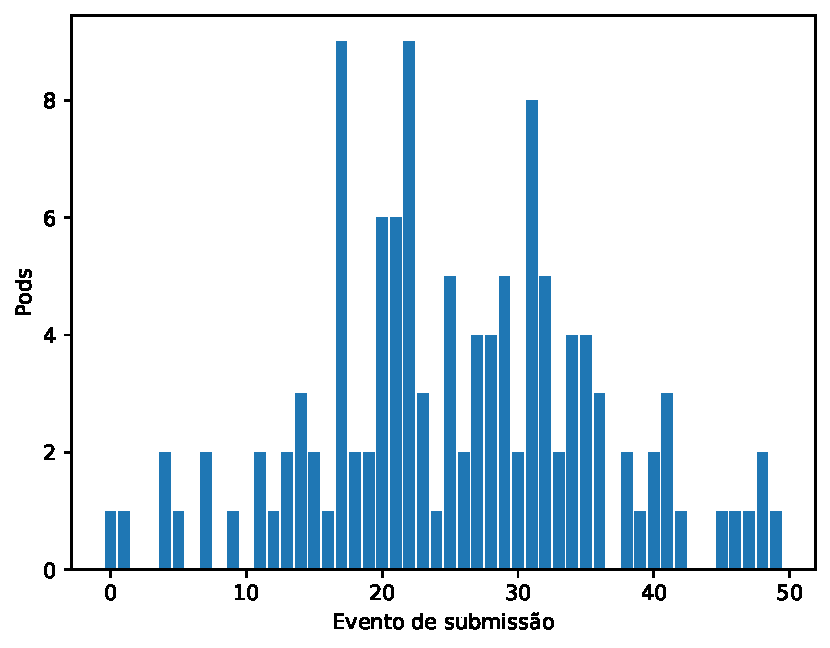
\includegraphics[width=.9\linewidth]{assets/workload-distribution.pdf}
	\legend{Fonte: O autor}
\end{figure}

O simulador de eventos também é responsável por injetar falhas do tipo \textit{crash} ao escalonador em execução. No \textit{Kubernetes}, todos os sistemas internos são representados por \textit{pods} (inclusive o \textit{Kube-Scheduler}), logo, a simulação de uma falha consiste em reinicializar de forma forçada o \textit{pod} responsável pelo escalonamento. Visando observar o comportamento dos escalonadores quando são submetidos a erros, foram desenvolvidos 2 cenários de falhas, denominados Moderado e Intenso. Os cenários de erros visam degradar as métricas de desempenho simulando falhas de escalonamento, no Moderado, ocorreu um disparo total de 5 falhas em eventos estratégicos de submissões de \textit{Pods}, isto é, os eventos 14, 27, 41, 52, 67. No cenário Intenso, há um total de 11 falhas distribuídas nos eventos de submissões 4, 9, 14, 17, 21, 25, 30, 33, 36, 38, 45. 

%O simulador de eventos também é responsável por disparar erros ao escalonador em execução. Uma simulação de erro consiste em derrubar o escalonador em execução, forçando a reinicialização do \textit{pod} que o representa. Serão utilizados 3 cenários de falhas durante as baterias de testes, com o objetivo de analisar as abordagens de escalonamento em diferentes cenários de falhas. Os cenários de falhas, ou \textit{profile}, é um reflexo do modelo padrão dos testes, entretanto, inserindo algumas simulações de falhas em certos eventos de submissão. Os profiles de falhas são denominados de Leve, Moderado e Intenso:
%\begin{enumerate}[label=(\alph*)]
%	\item Leve: 2 disparos de falhas nos eventos 21 e 61;
%	\item Moderado: 4 disparos de falhas, eventos  12, 30, 50 e 67; e
%	\item Intenso: 9 disparos de falhas, eventos 2, 12, 25, 31, 37, 45, 52, 62, 74.
%\end{enumerate}
Os disparos de falhas são executados após o evento de submissão de \textit{pods}. Por exemplo, a falha que está no evento 21 degradará o escalonamento a partir do evento 22. A Figura \ref{fig:profiles-erro} representa cada \textit{profile} sobreposto ao teste padrão de execução, onde as barras em vermelho são as injeções de falhas ao escalonador em execução.

\begin{figure}%
	\centering
	\subfloat[\centering Moderado]{{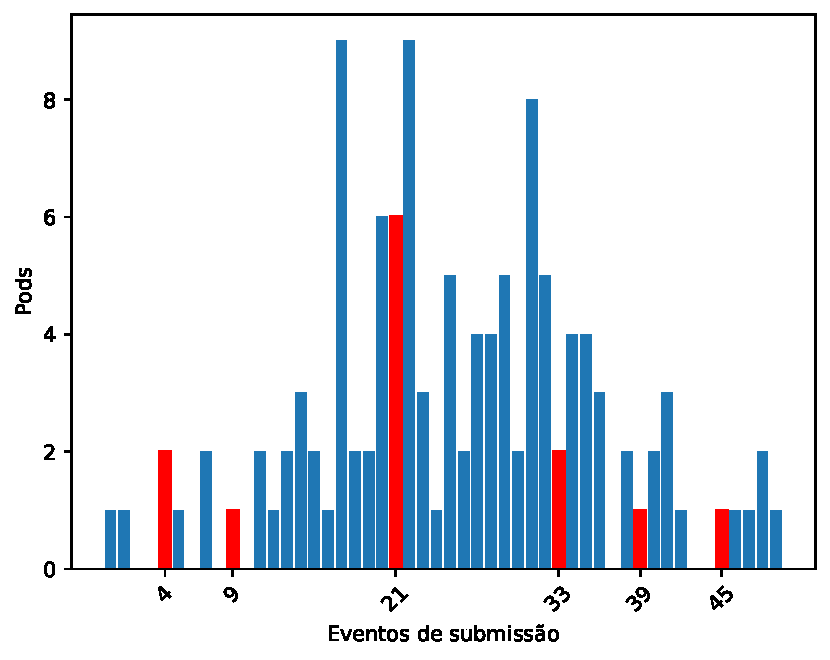
\includegraphics[width=.70\linewidth]{assets/error-moderado.pdf} }}%
	\qquad
	\subfloat[\centering Intenso]{{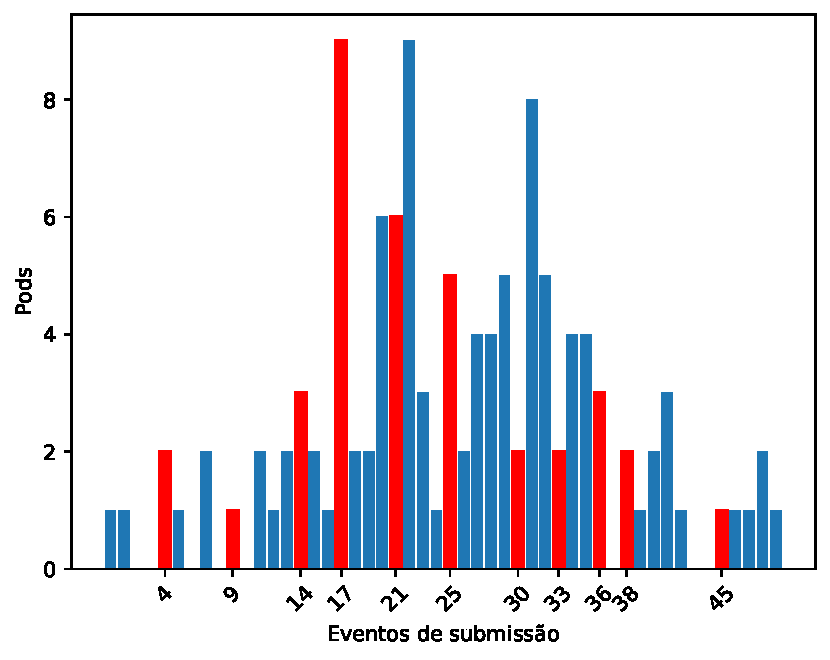
\includegraphics[width=.70\linewidth]{assets/error-intenso.pdf} }}%
	%\qquad
	%\subfloat[\centering Intenso]{{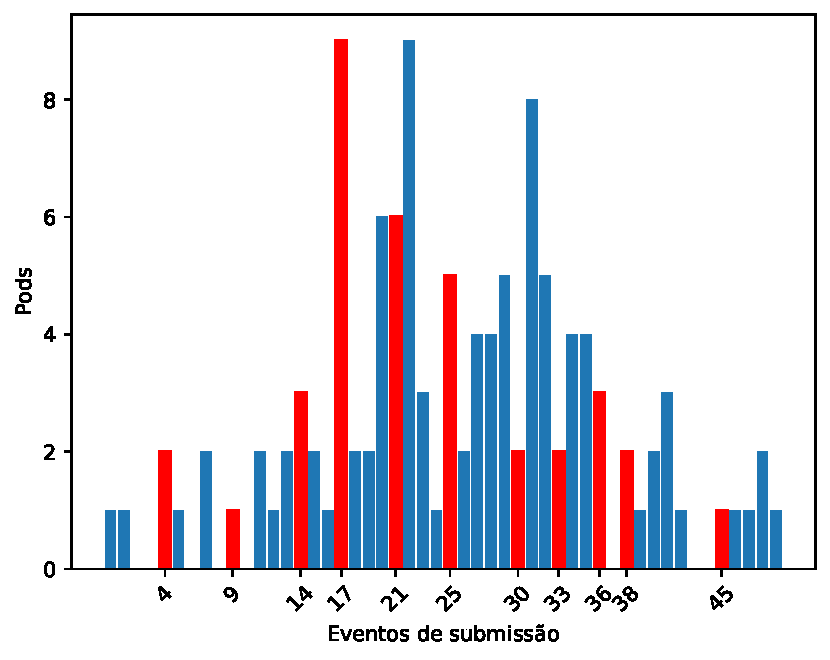
\includegraphics[width=.55\linewidth]{assets/error-intenso.pdf} }}%
	\caption{Cenários de falhas}%
	\label{fig:profiles-erro}%
\end{figure}

\section{Considerações parciais}

O presente capítulo apresentou um protocolo experimental para analisar o desempenho do escalonador proposto.
%
Dois cenários foram elaborados, denominados Moderado e Intenso.
%
Em suma, os cenários variam o número de falhas que ocorrem na infraestrutura computacional.
%
Por definição, as falhas sempre ocorrem em recursos que hospedam partes do escalonador.
%
Os resultados experimentais são apresentados no próximo capítulo, comparando o escalonador proposto no trabalho com as abordagens utilizadas como padrão na arquitetura \textit{Kubernetes} tradicional.
%TODO explicar o algoritmo de simulador de eventos
%TODO pseudocódigo
%TODO definir um profile fixo de disparo de erros























